% SPDX-FileCopyrightText: 2024 Lukas Zirpel <thesis+lukas@zirpel.de>
% SPDX-License-Identifier: GPL-3.0-only

\chapter{Methodology}
\label{chap:methodology}

This chapter details the methodology employed to evaluate the performance of various censorship evasion protocols under realistic network conditions.
We describe our experimental design, emphasizing the requirements.
The chapter then outlines the testbed setup, including the transition from a virtualized environment using the NixOS testing framework to a real-world hardware implementation.
Finally, we discuss the rationale behind our protocol selection, the specific network parameters varied during testing, and the data analysis pipeline used to process the collected packet captures, providing a comprehensive overview of our experimental approach.

\section{Experimental Design}
We want to measure the overhead of encryption and censorship evasion protocols over lossy links.
Therefore, we need a measurement setup, which allows us to do so, with repeatability and consistency.
It should also include a traffic generator, which generates the simplest possible traffic pattern, a constant stream of data.
The stream of data should only flow in one direction.
The traffic generator should not attempt to do congestion control, as we don't want our results to be influenced by the particular congestion control algorithm being used.
The setup should further allow simulating different network conditions.
Data traffic should flow from the traffic generator, be obfuscated and/or encrypted by the censorship evasion protocol, pass through the network emulator and finally be de-obfuscated and/or decrypted by the censorship evasion protocol.
All packets should be recorded in their original form with accurate time stamps.
If packets are recorded on multiple systems, special care needs to be taken to synchronize their clocks precisely.
Otherwise, calculating accurate time deltas as a packet traverses a path is practically impossible.
The packets can be analyzed later (post-experiment analysis) and the analysis pipeline can be iterated on without rerunning all experiments.
It should also be easy to add new protocols and experiment with the setup both for us and for future researchers wishing to tweak the setup or test more protocols.

\section{Testbed}
\begin{figure}[tbh]
	\centering
	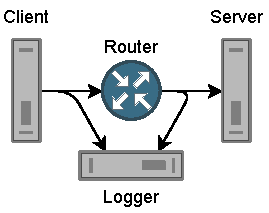
\includegraphics[draft=false,width=0.4\textwidth]{figures/Network schematic/actual/setup.pdf}
	\caption{Our Network Setup}
	\label{fig:actual_network_schematic}
\end{figure}
\begin{figure}[tbh]
	\centering
	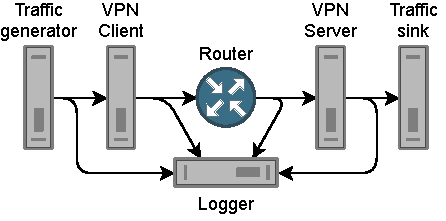
\includegraphics[draft=false,width=0.7\textwidth]{figures/Network schematic/optimal/setup.pdf}
	\caption{Improved Network Setup}
	\label{fig:optimal_network_schematic}
\end{figure}

As can be seen in \Cref{fig:actual_network_schematic}, our setup consists of four hosts.
The \textit{Client} runs iperf3 as a traffic generator in UDP mode, and the censorship evasion client software.
The \textit{Router} routes packets between the Client and the Server and emulates different network conditions, such as packet loss.
The \textit{Server} runs an iperf3 server instance and the censorship evasion server software.
The \textit{Logger} records all traffic seen on the link from the Client to the Router and from the Router to the Server.
We're capturing packets on a separate host to make sure the measurement does not influence the rest of the test setup, e.g., through higher CPU utilization of a host.
By creating all packet captures on a single host, we also remove the need for precise clock synchronization.

There are a number of existing network simulators for simulating complex network setups with routers, switches, etc. \cite{network-simulators-list}.
Many of them focus on simulating mesh networks for testing routing protocols, for example Mesh Network Lab \cite{meshnet-lab}.
Our network is relatively simple, while the complexity lies in the configuration of the hosts and automation.
This is part of the reason why we chose the NixOS testing framework for our first prototypes.
The other reason is that Nix has the desirable properties mentioned in \Cref{Nix-explanation}.
It allows declararing the exact configuration of the hosts and the virtual network in code.
All dependencies are pinned in a lock file and no outside dependencies are used, so everything should still be reproducible in a decade or more without having to distribute gigabytes of VM or container images and while still being able to easily modify any part of the system.

First, we use the NixOS testing framework for prototyping, and then transfer the setup to bare-metal hardware.
The NixOS testing framework launches several VMs with QEMU and sets up a virtual network switch.
Using the NixOS testing framework, we declare the configuration of all four hosts, as well as the network topology, in Nix code.
We also specify a test script, which imperatively executes one command at a time.
The script roughly executes these steps: start all hosts, wait for them to be ready, tell the router to emulate the network conditions we want, start the traffic generator, wait for it to be done, and finally collect the packet captures.
Different network conditions can be emulated using Linux's network emulator\cite{man8:tc-netem}.
iperf3 is run with the \texttt{-R} flag to simulate a download from the point of the client \cite{man:iperf3}.
We call the packets flowing from the server to the router \textit{pre} and the ones after the router \textit{post}.
All packet captures are stored for later analysis.

Since the virtualization may influence our results in unexpected ways, especially since all VMs are running on the same host and the network is only simulated, we opted to perform our actual measurements on bare metal hardware.
While it is definitely possible to build a reliable benchmarking setup using virtual machines, a virtual network switch and virtual networking cables, using bare metal hardware eliminates the virtualisation as a variable in our measurements.
For that, we installed NixOS on PCs, which are centrally controlled with a custom measurement harness.
nixos-anywhere \cite{nixos-anywhere} is used to quickly and reproducibly install the operating system on all machines.
nixos-anywhere uses disko \cite{disko} to partition and format the disks in a declarative way.
Our custom measurement harness is designed to be compatible enough with the NixOS testing framework to work with the same test script.
However, Nix is not really designed for this use case, and isolates the build steps in a sandbox with no network access and no access to SSH keys.
Normally, Nix expects to manage all dependencies by itself to ensure purity, but disabling the sandbox allows accessing things outside of the sandbox, which is impure.
Having real hardware in the loop and not just a simulation of that hardware is inherently impure and requires disabling the sandbox.
This allows using SSH to reach all the machines (and read the secret key) from within a nix build (nix derivation).
As a consequence, this action invalidates some of the guarantees that Nix normally provides.
When running the setup, the operator needs to make sure that the real world matches all assumptions of the test script.
This includes having an SSH secret key in the right location on the filesystem of the host controlling the tests, that the four machines are booted and allow access using the above key, that the operating systems running on the machines are configured perfectly by running the correct configuration, and that the network is configured correctly, including the configuration of the switch.

Despite Nix not really being designed for this particular use-case, we can still take advantage of all other Nix features.
We can use it as a simple templating engine to build the test script with the right parameters and then execute it.
Modifying any part of the pipeline ensures that only the modified and subsequent stages are rerun.
This eliminates the need for manually selecting which parts of the pipeline to run, a process that can be both tedious and error-prone, or rerunning the entire pipeline every time, which is time-consuming.
Furthermore, building our setup in this way allows using the same test script and data analysis pipeline for the VM tests and the hardware tests, which makes experimentation much easier.
We use Nix to take care of storing all packet captures and the build logs.
But if Nix were to get in the way for whatever reason after running the measurements, the data can still be easily copied out of the Nix store.
This can be done by specifying the measurements which should be exported in \path{test-matrix/parameters.json} and then running \mintinline{shell}{nix build .#measurements}.
The reason why we want to store the packet captures in the Nix store is for easy processing by the data analysis pipeline.
However, one potential downside of using Nix for this purpose is that care must be taken not to modify the test script or any other dependencies, as doing so would trigger the tests to run again.
This can also be seen as a positive feature, as it helps prevent modifications that are believed to not influence the results but actually do so.

In the VM test setup, the virtual switch is configured \cite{NixOS-VM-test-Hub} to behave like a hub \cite[Clause 12.4]{9844436}, which makes it easy to capture the packets on both VLANs.
On real hardware with a real switch, this is not quite as trivial.
To replicate this setup with real hardware, we use Cisco's Switched Port Analyzer (SPAN), also known as port mirroring \cite{cisco-span-tutorial}.
Since enabling SPAN disables our ability to transmit packets from that interface for management purposes, we use a USB to Ethernet adapter for the management interface.
The switch has several 100Mbit/s and 1Gbit/s Ethernet ports.
The client, router and logger are connected to 100Mbit/s ports, therefore limiting the bandwidth to 100Mbit/s.
During a measurement, data almost exclusively flows in one direction (apart from a small amount of iperf3 status information).
Therefore, the router being connected to the switch with 100Mbit/s full duplex is sufficient.
To record the data, we use port mirroring to copy the data being transfered on the port of the router, to the logger.
Since this can result in a maximum data rate of 200Mbit/s, the monitor port of the logger is connected to a 1Gbit/s switch port in order to keep up with the data rate.
iperf3 is configured to send at a rate of 100Mbit/s, since transferring data at a faster rate is not possible anyways.

An important consideration for real-world deployment of censorship circumvention tools is their resource consumption.
While we aimed to quantify both processing power and RAM requirements, direct measurement of RAM usage for WireGuard proved challenging, as there seems to be no simple and reliable way of measuring the RAM usage of a Linux kernel module.
We determine the CPU usage of WireGuard in a somewhat ad hoc way by looking at the output of
\begin{minted}{shell}
ps aux | grep wg-crypt | grep root | awk '{total+=$3;} END{print total;}'
\end{minted}
during a measurement with no network impairments.
The CPU usage of the other tunnel protocols is determined in a similar way.
For userspace programs running in systemd units, the RAM usage can be assessed using \mintinline{shell}{systemctl status}.

We gather the MTU of each tunnel interface from the output of the \mintinline{shell}{ip link} command.

\subsection{Hardware Used}
Detailed hardware information can be found in \Cref{tab:hardware}.
\begin{table}[tbh]
	\centering
	\footnotesize
	\begin{tabular}{cl}
		\toprule
		\textbf{Category} & \textbf{Details}                                                                                       \\ \midrule
		\rowcolor[HTML]{EFEFEF}
		Switch            & Cisco Catalyst 2960C-8PC-L                                                                             \\
		& 8 10/100BASE-T PoE ports                                                                               \\
		\rowcolor[HTML]{EFEFEF}
		& \begin{tabular}[c]{@{}l@{}}2 dual-purpose ports\\ (10/100/1000BASE-T copper and SFP) \cite{cisco-switch-hardware-installation-guide}\end{tabular}      \\
		& Cisco IOS Release 15.2(7)E8                                                                            \\ \midrule
		\rowcolor[HTML]{EFEFEF}
		PCs               & DELL OptiPlex 7070 Micro                                                                               \\
		& INTEL® CORE™ i5-9600 (6 cores, 3.1GHz)                                                                 \\
		\rowcolor[HTML]{EFEFEF}
		& \begin{tabular}[c]{@{}l@{}}16GB RAM\\ One 2666 MHz DDR4 SODIMM module,\\ HMA82GS6JJR8N-VK\end{tabular} \\
		& 512GB NVME SSD                                                                                         \\ \bottomrule
	\end{tabular}
	\caption{Hardware used}
	\label{tab:hardware}
\end{table}



\section{Scenario Selection}
\subsection{Protocols to test}

To evaluate censorship evasion protocols, we select a range of protocols representing different approaches and levels of sophistication.
Our selection includes:

\begin{itemize}
  \item \noindent\textbf{None (Baseline):}
    A baseline measurement with no protocol encapsulation provides a reference point against which the performance of the other protocols can be compared.
    This allows us to quantify the overhead introduced by each protocol.

  \item \noindent\textbf{WireGuard:}
    WireGuard is a modern, fast, and secure VPN protocol that utilizes state-of-the-art cryptography \cite{donenfeld2017wireguard}.
    It is known for its performance and ease of configuration, making it a popular choice for VPN applications.
    We include WireGuard to assess the impact of a well-optimized VPN protocol on network performance under challenging conditions.

  \item \noindent\textbf{DNS Tunnel (iodine):}
    DNS tunneling is a technique that encapsulates data within DNS queries and responses, allowing communication to bypass some forms of censorship.
    While less efficient than most other methods, it can be effective in bypassing certain types of firewalls that allow DNS traffic.
    iodine is a widely used implementation of DNS tunneling.
    We select iodine to investigate the performance characteristics of this technique, particularly its susceptibility to latency and packet loss.

  \item \noindent\textbf{ICMP Tunnel (ICMPTX):}
    ICMP tunneling uses ICMP echo requests and replies to carry data.
    ICMPTX is a common tool for ICMP tunneling.
    We include ICMPTX to examine the performance of this approach, especially in the context of lossy or high-latency networks.

  \item \noindent\textbf{Tor Pluggable Transports:}
    Tor is an anonymity network that relies on a network of relays to anonymize traffic.
    In places, where censors attempt to block access to Tor, users can use so-called \textit{Pluggable Transports} to circumvent the block.
    There are a variety of such protocols, with the most common ones being obfs4, Snowflake, and meek.
    We select these specific Tor protocols because they are known to be effective against censorship in the real world.
\end{itemize}



\begin{table}[tbh]
	\centering
	\footnotesize
	\begin{tabular}{ccccc}
		\toprule
		\textbf{\begin{tabular}[c]{@{}c@{}}Loss\\ {[}\%{]}\end{tabular}} & \textbf{\begin{tabular}[c]{@{}c@{}}Delay\\ {[}ms{]}\end{tabular}} & \textbf{\begin{tabular}[c]{@{}c@{}}Jitter\\ {[}ms{]}\end{tabular}} & \textbf{\begin{tabular}[c]{@{}c@{}}Duplicate\\ {[}\%{]}\end{tabular}} & \textbf{\begin{tabular}[c]{@{}c@{}}IPv4 Payload\\ {[}Bytes{]}\end{tabular}} \\ \midrule
		\rowcolor[HTML]{EFEFEF}
		0                                                                & 0                                                                 & 0                                                                  & 0                                                                     & 556                                                                         \\
		0.1                                                              & 1                                                                 & 10                                                                 & 1                                                                     & 1260                                                                        \\
		\rowcolor[HTML]{EFEFEF}
		0.2                                                              & 10                                                                &                                                                    & 10                                                                    & 1400                                                                        \\
		0.5                                                              & 50                                                                &                                                                    &                                                                       & 1480                                                                        \\
		\rowcolor[HTML]{EFEFEF}
		1                                                                & 100                                                               &                                                                    &                                                                       &                                                                             \\
		5                                                                & 200                                                               &                                                                    &                                                                       &                                                                             \\
		\rowcolor[HTML]{EFEFEF}
		10                                                               &                                                                   &                                                                    &                                                                       &                                                                             \\ \bottomrule
	\end{tabular}
	\caption{Sampling the Parameters}
	\label{tab:parameters}
\end{table}

To comprehensively evaluate the performance characteristics of the chosen censorship circumvention protocols under realistic network conditions, we varied the following parameters:

\noindent\textbf{Loss:} Packet loss is a common impairment in real-world networks, particularly in congested or unreliable environments.
We vary the packet loss percentage to assess the resilience of each protocol to data loss and its impact on throughput and latency.
A range of loss values is chosen to simulate conditions from mildly congested to severely impaired networks.

\noindent\textbf{Delay:} Network latency, or delay, refers to the time it takes for a packet to travel from source to destination.
High latency can significantly impact user experience, especially for interactive applications.
We vary the delay to measure how each protocol's performance is affected by increased round-trip times.
The delay is distributed according to a normal distribution over a range of delay ± jitter \cite{man8:tc-netem}.
A range of delay values is chosen to simulate conditions from low-latency to high-latency networks.

\noindent\textbf{Jitter:} Jitter is the variation in packet delay.
It can be even more disruptive than consistent latency, as many protocols (e.g., TCP) are sensitive to packet reordering.
We vary jitter to see how each protocol is influenced by fluctuating delays.

\noindent\textbf{Duplicate:} Packet duplication occurs when a packet is sent multiple times or copied on the way, often due to network issues.
Duplication wastes bandwidth and can cause confusion at the receiver.
We introduce some duplication to examine how each protocol handles duplicate packets and its effect on overall performance.

\noindent\textbf{IPv4 Payload:} The IPv4 payload size is the size of the payload inside the IP packet.
The full IP packet including header will be 20 bytes larger than this value for IPv4.
If any tunnel protocol is used, it will add more overhead.
The Maximum Transmission Unit (MTU) defines the largest size of a packet that can be transmitted over a network link.
We varied the IPv4 payload size to simulate the impact of different MTUs on the performance of each protocol.
A range of MTU values was chosen to simulate different network configurations and to evaluate the impact of fragmentation (or lack thereof) on performance.

When running measurements where we keep all parameters constant and only vary one at a time, there are $7 + 5 + 2 + 3 = 17$ measurements per protocol.
The execution time is bounded by the measurement duration, which is 5 minutes, so 17 measurements will take at least $17 * 5 m = 85 m = 1h25m$.

Since many link layer protocols employ error detection and correction algorithms, it is not common for packets to become corrupt in the real world but some protocols may still behave in unexpected ways.
While Linux's network emulator also supports corrupting packets in addition to all of the above parameters, we do not use this functionality.
The reason for this is described in \Cref{sect:data-analysis-pipeline}.

In order to save some space when storing the packet captures (\path{.pcap} files \cite{ietf-opsawg-pcap-04}), compression can be used to reduce the storage requirements.
The \path{.pcap} files only compress well if the data is not encrypted or otherwise scrambled too much.
The files could either be explicitly compressed with a file compression tool like zstd or the compression could be done at the filesystem level, e.g., with OpenZFS \cite{OpenZFS} and Btrfs \cite{Btrfs}.
We opt for the latter approach due to its simplicity and transparent operation.

Since we're only interested in measuring what happens during the actual test and not in the connection setup and teardown of iperf3, we employ heuristics to ignore this part of the packet capture.
To find the start of the test, we find the first packet which is larger than a threshold (400 bytes).
To find the end of the test, we find the last packet which is larger than the same threshold and also ignore all packets which are sent after the duration of the test is over.


\section{Data Analysis Pipeline}
\label{sect:data-analysis-pipeline}
First we run our measurement setup with a particular set of parameters.
All packets before (pre) and after (post) the router are recorded and stored in \path{.pcap} files.

For all packets, we extract the timestamp and size and compute the BLAKE3 \cite{BLAKE3} hash of the IP payload and write the information into a JSON \cite{RFC8259} file (done in \mbox{\path{analysis/parse/parse.py}}).

Next, for each pre-packet, we find the same packet post the router (done in \path{analysis/statistics/statistics.py}).
If we assume that all pre-packets are unique and that the router does not modify packets, then we can simply match pre- and post-packets based on their hash.
If a pre-packet has the same hash as a post-packet, then it is the same packet.
This way, we can determine if a packet was dropped, duplicated or simply forwarded normally.
If no matching post-packet matches for a particular pre-packet, it means that the packet was lost (dropped).
If more than one packet matches, it was duplicated.
If exactly one packet matches, it was routed successfully without duplication.
If the router were to corrupt a packet, then this approach would no longer work.
The assumption that pre-packets are unique seems to hold in practice, when not using any tunnel protocol, as iperf3 uses a monotonically increasing counter in each packet.
The assumption does however not hold when using a tunnel protocol which fragments packets into smaller fragments.
This is because with high probability, not many bits of the iperf3 counter value change from one packet to the next, resulting in a high probability of only one fragment being different.
Since there is an upper bound to the latency we simulate, it is sufficient for packets to be unique within a certain time window.
But in order to be robust against duplicate pre-packets being sent almost at the same time, a better algorithm needs to be developed.
One approach could be to match each post-hash to its closest (in time) matching pre-hash.
For meaningful statistics over time, we group the data into short chunks (buckets) of one second each and compute bandwidth and packet counts over that bucket.
The latency introduced by the router can be measured by computing the difference between the timestamps of each pre-packet and the first corresponding post-packet.
For our latency statistic, dropped packets are ignored and for duplicated packets only the first arriving packet is counted.
Throughput can be measured by summing up the IP payload size in every bucket and dividing it by the time duration of the bucket.
This meaurement of throughput includes the overhead of the tunnel protocol.
If the overhead is fixed and known for a given tunnel protocol, we can compute the goodput (actually useful throughput inside the tunnel), by simply subtracting the overhead from the packet size before computing the throughput.
For our throughput statistic, dropped packets don't count and packets which were duplicated count only once.
The output of this analysis step is a JSON file with the following contents:
For each bucket, we store the center timestamp of the bucket, packet counts (dropped, duplicated and normal), throughput and a the latency of each packet.

Finally, we render graphs from the data using Matplotlib \cite{Matplotlib} (done in \path{analysis/graph/graph.py}).
For looking at the metrics from one particular measurement over the course of the measurement, we create several graphs (see \Cref{sect:graphs-single}).
Since we're usually more interested in observing how certain metrics differ between measurements with different parameters, we implemented the ability to show multiple measurement runs in one graph.

Showing all metrics over time for all different measurements would become too confusing as many lines overlap, making the graph too visually busy.
Instead, we remove the time component and show violin plots of the metrics.
For that, we first collect all the buckets into one and then render the data into graphs (see \Cref{sect:graphs-multi}).


%%% Local Variables:
%%% TeX-master: "thesis"
%%% End:
